\chapter{Introduction}\label{chap:introduction}
In recent years there has been a large increase in so-called \emph{smart devices}. 
A smart device is an electronic device that is connected to one or more other smart devices. 
Common protocols for the interconnection of smart devices are WiFi and Bluetooth, among others.
Smart devices are part of a concept called the Internet of Things, or IoT. 
IoT is a network of physical devices, 
where the devices have unique identifiers and are connected to the Internet, 
making them accessible from other devices such as personal computers or smartphones. 
Example of devices that are part of a network could be an air condition unit, a coffee machine, a watch or a refrigerator. 
Devices such as smartphones, laptops or servers, 
that are already commonly connected to the Internet, 
are usually not considered part of the IoT network. 

We will in this chapter gain an insight of what is the current state of \emph{wearables} and \emph{smart homes}. 
We first describe the initial problem in \Cref{sec:initproblem}, 
which describes what information we are looking to explore and why. 
After describing this problem, 
we analyze wearables, \ie smart devices that are worn, in \Cref{sec:wearables}.
Another large part of IoT is the concept of smart homes, 
\ie homes that are controlled or automated by utilizing smart technologies and devices. 
We will analyze smart homes in \Cref{sec:smarthomes}, 
where \Cref{sec:system-categories} describes different levels of home automation. 
Then we propose a problem statement \Cref{sec:researchstatement}, 
and describe our target group in \Cref{sec:target-group}.
We describe a list of requirements for our solution in \Cref{sec:requirements-specification},
and give an overview of the rest of the report in \Cref{sec:overview}.

\section{Initial Problem}\label{sec:initproblem}
Wearable technology is a trending form of technology as of 2015 \cite{WEARABLESTREND}. 
As the name implies, wearables are devices that, 
unlike most electronics, are worn by the user. 
As shown by \Cref{fig:wearables-placement}, 
the most common type of wearables today are wrist-worn, 
\eg smartwatches or smart-wristbands (such as fitness trackers).
Smartwatches are watches that run an advanced operating system, 
and can perform more actions than regular watches, 
such as communicating with a smartphone or other smart devices.
Smart-wristbands are typically fitness trackers which track activity, among other things, 
and send this data to a connected smartphone via an application. 
Smartphones are usually not considered a wearable since they are \emph{carried} and not \emph{worn}. 

\begin{figure}[!htb]
  \centering
  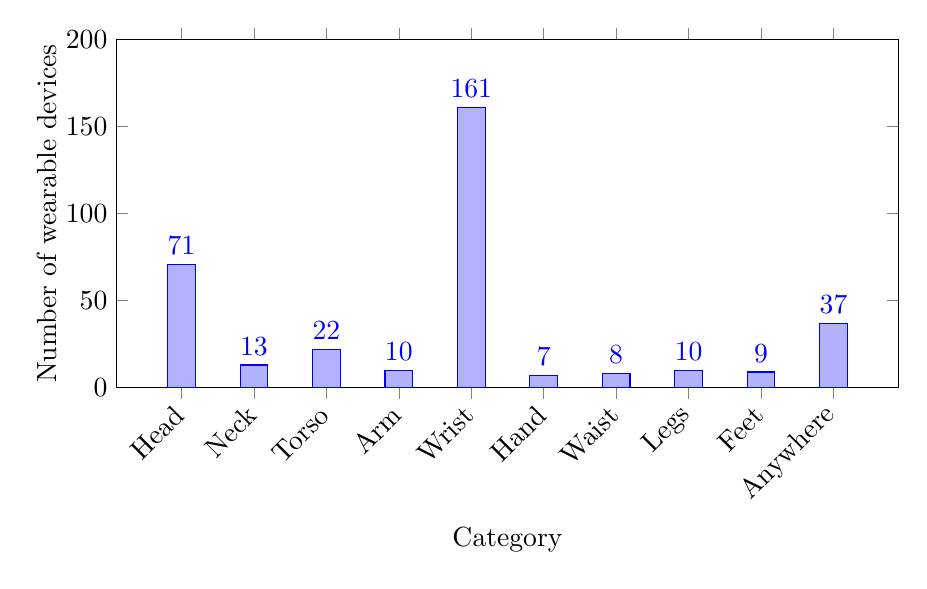
\begin{tikzpicture}
\begin{axis}[
    height=6cm,
    width=0.95\textwidth,
    xlabel={Category},
    xticklabel style={rotate=45, anchor=east, yshift=-0.5ex},
    ylabel={Number of wearable devices},
    yticklabel style={align=right,inner sep=0pt,xshift=-0.3em},
    nodes near coords align={vertical},
    nodes near coords,
    xtick=data,
    symbolic x coords={Head,Neck,Torso,Arm,Wrist,Hand,Waist,Legs,Feet,Anywhere},
    ybar,
    ymax=200,
    ymin=0,
    ]
    \addplot coordinates {(Head,71) (Neck,13) (Torso,22) (Arm,10) (Wrist,161) (Hand,7) (Waist,8) (Legs,10) (Feet,9) (Anywhere,37)};
\end{axis}
  

\end{tikzpicture}
  \caption{Placements of wearables. Data from \protect\cite{LISTOFWEARABLES}.}
  \label{fig:wearables-placement}
\end{figure}

The increasing trend in wearables is likely due to increased computational power in small devices, 
and decreased sizes of sensors, 
which allows more power and functionality to wearables devices. 
This increasing trend, as well as better wearables devices, 
opens up new possibilities since we can now carry more computational power with us on the go, 
which we can utilize to perform actions that we could not before, 
or perform actions faster or better. 
An example of this is that we can now track our level of activity, 
together with our location to analyze ourselves, 
or even automate actions based on our location, mood or even health. 

Another trend that utilizes IoT is smart homes.
Smart homes are homes that are to some degree automated by utilizing IoT devices. 
The devices used for smart homes differ from wearables as they are usually stationary. 
The concept of smart homes has been around since the 1960's, 
where ``wired homes'' were built by hobbyists\cite{harper2003}. 
The first official use of ``Smart house'' was in 1984, 
by the American Association of Housebuilders \cite{harper2003}.

An extreme example of a high-end smart home is Bill Gate's mansion in Medina, Washington \cite{billgatehouse}.
This \$100 million house, finished in 2005, 
has sensors to adjust each room's temperature and lighting, 
and has speakers behind the wallpaper that follow you from room to room. 
The artwork in the house is mostly digital and can be changed by pressing a button. 
One can only imagine what other technology is being used in that house. 

With these increasing technology trends in wearables and smart homes, 
it could be very interesting to see how and if we can integrate these. 
It could be interesting to see if we can use wearables as a form of control of smart homes, 
or maybe even use wearables to automate the smart homes.
In the following sections we will look into the current state of wearables and smart homes, 
and investigate if we can integrate them. 

\section{Wearables}\label{sec:wearables} %Working title
%Thalley: Første source kan også laves som en fin graf hvis ønsket. Brug tal fra: http://www.statista.com/statistics/259372/wearable-device-market-value/
Wearable technology is a trending form of technology as of 2015 \cite{WEARABLESTREND}. 
As the name implies, wearables are devices that, unlike most electronics, are worn by the user. 
The most common types of wearables today are smartwatches, 
\ie watches that run an advanced operating system and can perform more actions that regular watches such as communicating with a smartphone or other smart devices, 
and smart wristbands which usually tracks activity, 
among other things, and sends this data to a connected smartphone via an application. 
Smartphones are usually not considered a wearable since they are usually \emph{carried} and not \emph{worn}. 

%Hvorfor wearables?
The increasing trend in wearables is likely due to increased computational power in small devices and decreased sizes of sensors, 
which allows more power and functionality to wearables devices. 
The increasing trend, as well as better wearables devices, 
opens up new possibilities since we can now carry more computational power with us on the go that we can utilize to perform actions that we could not before, 
or perform other actions faster or better. 
Examples of this could be that we can now track our level of activity together with our location to analyze ourselves or even automate actions based on our location, mood or even health. 

%HVad kan en wearable? Hvilke sensorer findes der? Hvad er state of the art? 
If we take a look at some of the current state of the art or the most popular wearable devices right now, 
we can create an image of what we can actually monitor, track, control or in other ways do with devices that we can wear. 
One of the latest and most advanced wearable is the HIRIS \cite{hirisweb}. 
The HIRIS is a wearable computer able to track 3D movements in real-time. 
By using several HIRIS, you can get a create a full-body tracking system. 
Aside from 3D tracking, HIRIS also tracks heart rate and temperature and can connect to other devices and control these. 
Another advanced wearable tracker is the Jawbone UP3 \cite{JAWBONE}. 
This wearable is also able to track your heart rate, activity, sleep and temperature, but unlike the Hiris cannot control any other devices. 
Since one of the most popular wearables is the smartwatch, it makes sense to mention these as well. 
One of most interesting smartwatches, due to developer options, is the Pebble Smartwatch \cite{PEBBLE}. 
This smartwatch works with iPhones and Android smartphones and comes with a variety of applications for tracking fitness and control music among other things. 
Aside from this, the watch also comes with an accelerometer and a magnetometer, meaning that is can track your motions and directions. 

By analyzing the list of 348 different wearables from Vandrico\cite{LISTOFWEARABLES} of September 2015, 
we can see which sensors and components are most common among wearables and where on the body they are worn. 
It is important to note that all of this information comes Vandrico's database, and may differ from other findings. 
\Cref{fig:wearables-category} shows which categories these wearables fit in. The most common one, lifestyle, 
describes wearables such as smartwatches or other devices that are meant to be used and worn on a daily basis. 
Some devices may fit more than one category.

\begin{figure}[!htb]
    \centering
    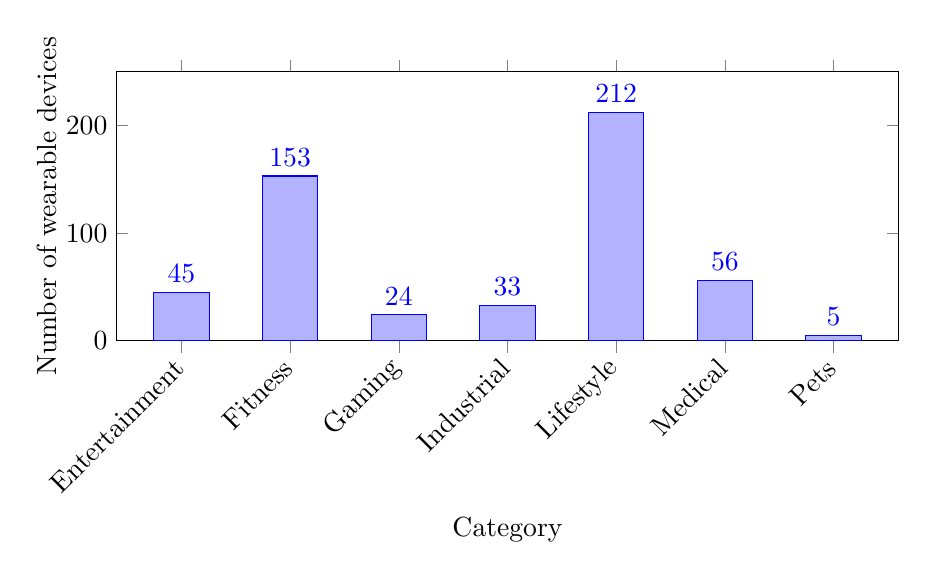
\begin{tikzpicture}
    \begin{axis}[
        height=5cm,
        width=0.95\textwidth,
        xlabel={Category},
        xticklabel style={rotate=45, anchor=east, yshift=-0.5ex},
        ylabel={Number of wearable devices},
        yticklabel style={align=right,inner sep=0pt,xshift=-0.3em},
        nodes near coords align={vertical},
        nodes near coords,
        xtick=data,
        symbolic x coords={Entertainment,Fitness,Gaming,Industrial,Lifestyle,Medical,Pets},
        ybar,
        ymax=250,
        ymin=0,
        bar width=20pt,
        ]
        \addplot coordinates {(Entertainment,45) (Fitness,153) (Gaming,24) (Industrial,33) (Lifestyle,212) (Medical,56) (Pets,5)};
    \end{axis}
\end{tikzpicture}
    \caption{Number of devices in each category}
    \label{fig:wearables-category}
\end{figure}

\Cref{fig:wearables-placement} shows where on the body the wearable should or can be worn. 
The most common placement is the wrist where smartwatches or wristband are worn, 
which are the most popular wearables. The devices that are worn on the head are usually augmented/virtual reality headsets, 
but also includes smart bike-helmets or ear/headphones.

\begin{figure}[!htb]
    \centering
    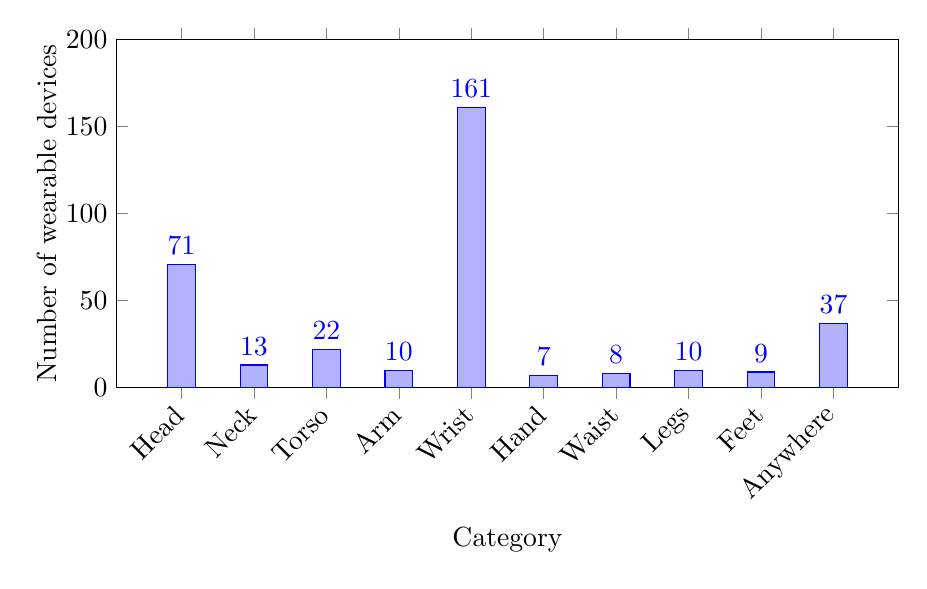
\begin{tikzpicture}
\begin{axis}[
    height=6cm,
    width=0.95\textwidth,
    xlabel={Category},
    xticklabel style={rotate=45, anchor=east, yshift=-0.5ex},
    ylabel={Number of wearable devices},
    yticklabel style={align=right,inner sep=0pt,xshift=-0.3em},
    nodes near coords align={vertical},
    nodes near coords,
    xtick=data,
    symbolic x coords={Head,Neck,Torso,Arm,Wrist,Hand,Waist,Legs,Feet,Anywhere},
    ybar,
    ymax=200,
    ymin=0,
    ]
    \addplot coordinates {(Head,71) (Neck,13) (Torso,22) (Arm,10) (Wrist,161) (Hand,7) (Waist,8) (Legs,10) (Feet,9) (Anywhere,37)};
\end{axis}
  

\end{tikzpicture}
    \caption{Placements of wearables}
    \label{fig:wearables-placement}
\end{figure}

\Cref{fig:wearables-sensors} shows which sensors and components are mostly available in wearables. 
Due to its high usability, the accelerometer is a very important sensor which is found in approximately half the wearables. 
The remaining sensors in \Cref{fig:wearables-sensors} are, unsurprisingly sensors that we also find in smartphones as they give a lot of options when it comes to developing applications. 
\begin{figure}[!htb]
    \centering
    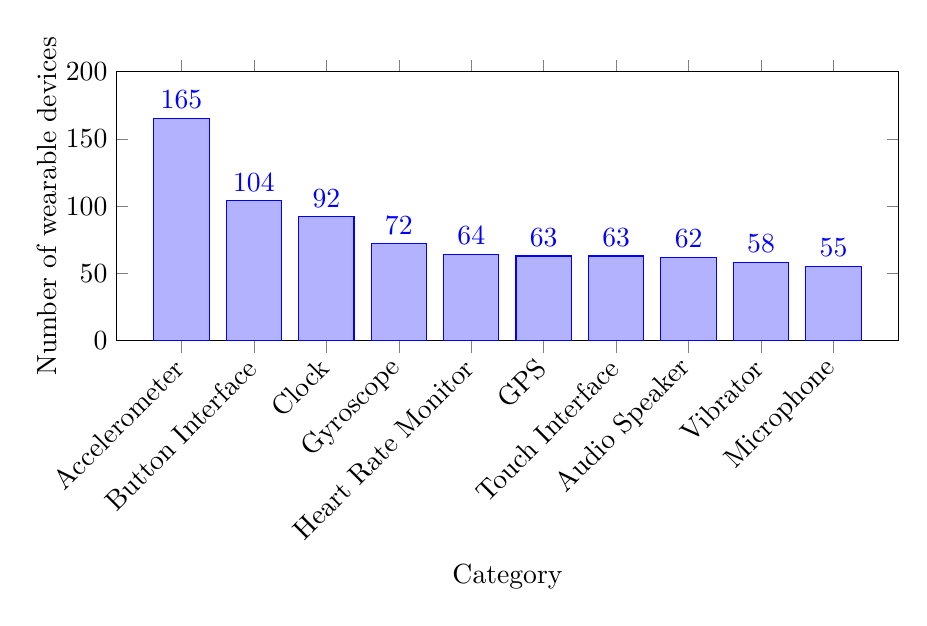
\begin{tikzpicture}
    \begin{axis}[
        height=5cm,
        width=0.95\textwidth,
        xlabel={Category},
        xticklabel style={rotate=45, anchor=east, yshift=-0.5ex},
        ylabel={Number of wearable devices},
        yticklabel style={align=right,inner sep=0pt,xshift=-0.3em},
        nodes near coords align={vertical},
        nodes near coords,
        xtick=data,
        symbolic x coords={Accelerometer,Button Interface,Clock,Gyroscope,Heart Rate Monitor,GPS,Touch Interface,Audio Speaker,Vibrator,Microphone},
        ybar,
        ymax=200,
        ymin=0,
        bar width=20pt,
        ]
        \addplot coordinates {(Accelerometer,165) (Button Interface,104) (Clock,92) (Gyroscope,72) (Heart Rate Monitor,64) (GPS,63) (Touch Interface,63) (Audio Speaker,62) (Vibrator,58) (Microphone,55)};
    \end{axis}
\end{tikzpicture}
    \caption{Top 10 mostly used sensors}
    \label{fig:wearables-sensors}
\end{figure}

This section gave a short overview of the current state of wearables, what they are and which sensors are widely available. 
This information should be remembered if developing any system that utilizes wearables. 

%Skab et overblik over de nyeste devices
%Grafer over hvilke sensorere der mest typiske?
%Grafer over kropsdele?
%Hvad er de nyeste teknologier indenfor wearables? 

\section{Smart Homes}
Another trend that utilizes the concept of IoT is smart homes which are homes that are, 
to some degree, automated by utilization IoT devices. 
The devices used for smart homes differ greatly from wearables as they are usually stationary. 
The concept of smart homes have been around for a while and numerous homes have already integrated some of these smart devices. 
A good example of a high-end smart home is Bill Gate's mansion in Medina, Washington \cite{billgatehouse}.
This \$100 million house have sensors to adjust each room's temperature and lighting, 
and have speakers behind the wallpaper that follows you from room to room. 
The artwork in the house is mostly digital and can be changed by pressing a button. 
One can only imagine what other technology is being used in that house. 

However, that is a rather extreme example of a smart home. 
Ordinarily, the devices found in smart homes are common items that has been connected to the Internet for wireless control.
Common devices that are found in smart homes include, but are not limited to, 
coffee machines, washers and dryers, thermostats, sound systems and locks. 
However, only few devices have really gained ground for the common user and few homes are automated.
One of the most commonly found IoT in homes are the Nest thermostat \cite{NEST}. 
This thermostat senses when you are around and when you are not to control the climate inside to save energy and thus money.
Unlike a lot of smart devices that are made to make your life a little easier, such as an automated coffee machine, 
the Nest thermostat helps you save money which is likely the reason for it popularity. 
Furthermore, the newest version (as of October 2015) allows you to connect other IoT devices to the thermostat. 
The Nest thermostat is thus starting to solve what is probable the greatest problem with smart homes (and IoT in general), 
and why they have not become popular yet: Lack of interconnectivity between IoT devices. 
This problem leads us to what is known as smart hubs. 

\subsection{Smart Hubs}
A smart hub is a device, or service, that implements several communication protocols used by IoT devices, 
and gives the user a single protocol or interface. 
The goal of a smart hub is to make the connected devices able to communicate. 

\subsubsection{Common Protocols for IoT}
\todo[author=Thalley]{Insert figure illustrating this}
There is a range of different protocols that are being used for various smart devices. 
We will not get into much detail with these protocols, 
but we demonstrate how many different there are and why communication is a problem.
\begin{table}
   \begin{description}
       \item[Protocol:] ZigBee
       \item[Used by:] Samsung, Jasco, Smartenit, FortrezZ and others
       \item[In products:] SmartThings Hub, thermostats, door sensors, light bulbs, etc.\\
       
       \item[Protocol:] Z-Wave
       \item[Used by:] FortrezZ, GE, Intermatic, Leviton, Aeon Labs, Evolve and others
       \item[In products:] Thermostats, wall outlets, door locks, door and window sensors, etc.  \\
       
       \item[Protocol:] WiFi (IEEE 802.11)
       \item[Used by:] Nest, Philips, Samsung, Bose, D-link and others
       \item[In products:] Thermostats, speakers, light bulbs, motion sensors, fitness trackers, camera, etc. 
    \end{description}
    \caption{Protocols used by various IoT devices}\label{table:iotprotocols}
\end{table}

Aside from the protocols in \Cref{table:iotprotocols}, 
there are several others messaging protocols such as MQTT, CoAP and XMPP used by various devices. 

A smart hub should thus not only be able to communicate with the devices, 
but also be able to transform the data to a single format and give easy access to it. 

\subsubsection{Smart Hubs on the Market}
The requirements for smart hubs have gained the attention of several large companies and even more smaller companies, 
all competing to be center of future smart homes. 
One of the mature commercial available smart hubs is the Samsung SmartThings Hub\cite{SMARTTHINGS}. 
The SmartThings Hub is a standalone device that supports the Z-Wave, ZigBee and WiFi protocols, 
and provides a smartphone application or a Representational State Transfer (REST) interface. 
The SmartThings Hub has been tested and is compatible with more than 150 devices as of October 2015,
but with support for the aforementioned protocols and a REST interface, this number is in practice higher.  
The price for such a hub is \$99, which is, compared to the prices for some of the compatible devices, very affordable. 
A more detailed description of the Samsung SmartThings Hub can be found in \Cref{sec:smartthings}. 

Samsung is, however, not the only company selling smart hubs. 
Microsoft has been working on their HomeOS\cite{HOMEOS}, Apple has their HomeKit\cite{HOMEKIT} and Google recently announced Brillo\cite{BRILLO}. 
While these products differ in terms of architecture, descriptions (operating system contra hub) and availability,
they all share the same goal of giving a centralized control of smart devices. 

There are also other open source alternatives such as openHAB\cite{OPENHAB}, 
where you simply setup your own server running the open sourced code and control the devices through that. 
The advantage here is of course the price (free) and the possibility of adding new unsupported products. 

\Cref{table:smarthubs} gives a short overview of some of the available or coming smart hubs. 
\begin{table}
    \centering
    \begin{tabular}{l l}
        Company                           & Product                              \\\hline
        openHAB\cite{OPENHAB}             & Employ open source code on own server \\
        Open Source Automation\cite{OSA}  & Employ open source code on own server \\
        OpenRemote\cite{OPENREMOTE}       & Employ open source code on own server \\
        Apple\cite{HOMEKIT}               & HomeKit Framework \\
        Samsung\cite{SMARTTHINGS}         & SmartThings Hub: A standalone device that cost \$99 \\
        Microsoft\cite{HOMEOS}            & HomeOS: An Operating system that runs on a server \\
        Google\cite{BRILLO}               & Project Brillo: An Operating system that runs on a server
    \end{tabular}
    \caption{An overview of home automation hubs from different companies}
    \label{table:smarthubs}
\end{table}

\subsection{Control of Smart Homes}
While smart hubs let different smart devices communicate, 
they are not meant to be a control panel for smart homes (although some, such as HomeOS, is designed as such).
To control the devices connected to a smart home, or standalone smart devices, 
most vendors offer some sort of smartphone application that gives the consumer a basic interface to control the device, set rules for it and so on.
This is for example the case with the Samsung SmartThings hubs. 

An alternative to such an application could be the Logitech Harmony Remote\cite{HARMONYREMOTE}, 
which is a universal remote that can connect to over \num{270000} devices (smart and dumb). 
It comes either as a standalone remote control or connected with a hub. 

Gesture control is a newer and more advanced way of controlling a smart home. 
A company known as Reemo\cite{Reemo}, formerly Playtabase, has created a way of controlling smart devices by gestures. 
They have developed a wearable devices, located on the wrist, that allows user to point at a device, 
and then perform a pre-programmed gesture that corresponds to a certain action for that device. 
A small received has to be placed near the devices that you want to control, 
and it is this received that you have to point to as depicted by \Cref{fig:reemo}. 
The pointing will, however, only work if the device is within line of sight. 

\begin{figure}[!htb]
    \centering
    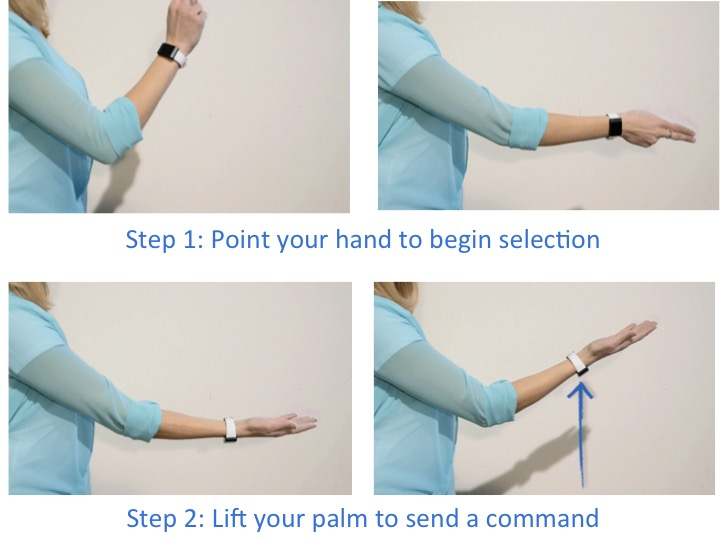
\includegraphics[width=0.8\textwidth]{images/Reemo}
    \caption{How Reemo gesture control works. Source: \url{http://www.getreemo.com/projects/}}
    \label{fig:reemo}
\end{figure}

Unfortunately they have not disclosed any details regarding the technology, 
how the receivers know which receiver you are pointing at or how the devices are controlled. 
The company and the product is also still in a development phase, 
so the product is not commercialized yet but have been in development since mid-2014.

These are the most common and/or most intuitive ways of controlling smart devices. 
The question is which is ``the best'', or rather, which method is the wanted way of controlling the devices.
\Cref{tbl:smartcontrol} summaries the aforementioned 3 ways. 

\begin{table}[!htb]
    \centering
    \parbox[t][][t]{0.3\textwidth}{
        \textbf{Smartphone application}\\
        \textbf{Pros:} Easy control of smart devices if the smartphone is usually carried or always near. 
                       Applications are usually available from vendors. 
                       Easy to get updates to the software. \\
        \textbf{Cons:} Requires a smartphone nearby to control. 
                       An overhead of unlocking phone, opening application and selecting device and action.
    }\quad
    \parbox[t][][t]{0.3\textwidth}{
        \textbf{Remote Control}\\
        \textbf{Pros:} Easy control of smart devices if the remote is usually carried or always near. \\
        \textbf{Cons:} Requires a remote control nearby to control (usually not very expensive). 
                       An overhead of selecting device and action.
    }\quad
    \parbox[t][][t]{0.3\textwidth}{
        \textbf{Gesture Control}\\
        \textbf{Pros:} Wearables are usually worn and grants easy control of applications by gesture.
                       Intuitive way of controlling devices (gestures imitates regular actions).
                       Easy to get updates to the software. 
                       No overhead of opening an application\\
        \textbf{Cons:} Requires a wearable to control. 
                       Have to remember gestures.
                       Must be in line of sight. 
    }
    \caption{Ways of controlling smart devices}
    \label{tbl:smartcontrol}
\end{table}

Each way has its pros and cons. 
A survey of 37 people showed that \perc{76} found gestures to be a natural way of controlling devices, 
while \perc{8} found it unnatural and the remaining left the question unanswered\cite{Kela2006}. 
This survey shows that users would rather have gesture for control, 
rather than the bother of always using their smartphone or remote for control.  
A product such as Reemo is a good way of controlling smart devices. 
However, as mentioned, it has a downside that the objects have to be in line of sight. 
If this restriction could be removed, it would improve this method. 

%%% Local Variables:
%%% mode: latex
%%% TeX-master: "../../master"
%%% End:

\section{Levels of Smart Home Automation}\label{sec:system-categories}
\todo[author=Thalley]{Bør vi ændre det med categories til noget med levels i stedet?}
Smart home automation is one of the big sell-points of smart homes.
Home automation can happen at various degrees. 
In this section we will analyze and categorize the different types of smart home automation. 
We divide the scenarios in which home automation is facilitated, 
into the following three categories:

\begin{enumerate}
    \item Rule driven systems
    \item Gesture driven systems
    \item Autonomous systems
\end{enumerate}

``Manual systems'' could constitute a fourth category, consisting of regular systems with manual switches,
but is left out as it such systems do not contribute to home automation.
The categories varies in the way users configure and interact with the systems. 
All the systems are, however, all driven by a set of \emph{rules}. 
The main difference is how the rules are defined or how they are used.
Each of the three categories and their use cases are briefly described below,
as well as how they can be integrated with wearables.

\subsection{User Defined Rule Systems}

These types of systems have a set of \emph{used defined} rules, 
that controls what the system does when certain events happen. 
The user defined rule systems use conditional statements to express input and output. 
Below are a few examples of rules in the form of (if this) \textrightarrow~(then that):

\begin{itemize}
    \item (The temperature is above 23 degrees Celsius) \textrightarrow~(Turn on the air conditioner)
    \item (The CO\textsubscript{2} index is critically high) \textrightarrow~(Open my windows)
\end{itemize}

The above rules consist of a condition on the left-hand side of the arrow, 
and an action on the right-hand side of the arrow.
The automation of the smart home is based on the set of rules. 
To achieve the desired behavior, the user must add, remove or tweak existing rules.

Examples of user defined rule systems include the aforementioned Apple HomeKit. 
As outlined in the framework reference for HomeKit \cite{applehomekitref}, 
the system is based on actions and events. 
Triggers constitutes rules by encapsulating actions and events. 
Each event represents a condition. 
An event may be fulfilled by a change in time, 
the state of devices in the system of the location of the user.

A wearable here could be integrated as a form of sensor (to \eg measure body temperature or CO\textsubscript{2} index), 
and use this information to perform the actions based on the rules.
Wearables could also be used to create a ``Follow Me'' system, 
that could track if the user is near \eg a door, and automatically open the door for the user. 

\subsection{Interactive Systems}

Interactive systems are explicitly controlled by the users, but in a smart way. 
Two main examples of interactive systems are gesture controlled and remote controlled. 

The gesture controlled systems are controlled by tracking the user's movements, 
and perform certain actions based on the movements.
Each device in the system responds to a set of gestures. 
For example, a lamp may respond to the user waving in order to turn on, 
and the user clapping in order to turn off.

A gesture driven system is partly a user defined rule system, 
as each gesture registered in the system is associated with one or more actions.
The association means that each time the gesture is registered in the system, the action should be triggered. 
Such rules can be formulated as ``if I wave, then lower the temperature on my thermostat'
The difference between these types of systems and the user defined rule systems, 
is that the actions are performed explicitly by the user, 
and not by measurements or other observations.

Examples of gesture driven systems include the aforementioned Hiris and Reemo, 
where wearables are used as active control units by performing gestures. 

The other type of interactive systems are the remove controlled systems. 
In these types of systems, the user controls the devices in the smart home using a remote control. 
The remote control could be the aforementioned Logitech Harmony Remote, 
but could also simply be a smartphone application. 
These types of systems are usually not combined with wearables, 
as they typically require a screen to control which device to perform an action on. 

\subsection{Autonomous Systems}

An autonomous system monitors the system, 
and proactively responds to changes in the system. 
Observable changes include but are not limited to changes in the temperature, 
CO\textsubscript{2} index, the number of people in the room or even who are in the room.
Autonomous systems should intelligently react to the users needs, 
based upon the observable state of the environment.

Autonomous systems rely on the concept of ambient intelligence, 
in order to determine the necessary actions.
\todo[author=Thalley]{Maybe add something about ambient intelligence here?}
Such systems include autonomous enhancement services, 
that replaces manual care with an automated system \cite{nehmer2006living}. 
These systems gather environment and user data, 
to determine the user's future actions or intentions. 
The autonomous systems are designed to what the users' want, 
without the users input or interaction. 
These systems applies methods and theories of statistics and machine learning, 
in order to learn the users behaviors and how to determine what the users want. 
For example if a user usually makes coffee in the morning, 
the system learns this routine and can then start the brewing process, 
when it measures that the user is waking up in the morning. 
%Thalley: Bedre eksempel ville være nice

Autonomous systems depend on rules like the previous two systems mentioned. 
The main difference here is that autonomous system create these rules \emph{themselves}, 
from observing the users and the environment, 
or with some preprogrammed rules defined by \emph{experts}
The rules of such systems are typically much more complex however. 
It is not given that users themselves are capable of determining a suitable set of rules, 
in order to \eg judge if their health is critical. 

\todo[author=Thalley]{Try to find a better reference for autonomous systems}
Examples of autonomous systems include the one described by Nehmer \etal \cite{nehmer2006living}. 
The authors envision a living assistance system which monitors elderly people. 
A model is outlined, 
and by continuously feeding the model with data about the individuals body functions and his behavior, 
they can determine if a \emph{critical situation} occurs. 
A critical situation could be that the person has fallen and is not responding to contact, \eg calls.
Such system may reduce the cost of providing care to the elderly people.

Wearables can play a huge part in autonomous systems. 
Previously mentioned in this report, 
wearables are able to measure a lot of different data about the environment (\eg room temperature, CO\textsubscript{2}, etc.), 
and the user (\eg body temperature, heart rate, movements). 
The reason why wearables especially plays a large role here, 
is not only the different types of data, but also the amount of it,
assuming that the user is wearing the measuring wearables most of the time. 

By using this data and statistics, the system can detect certain events or situations, 
such as knowing when the user is awake or asleep or maybe even detect the level of sleepiness or mood.    
Based on the data from wearables can be used to automate a lot of processes, 
and a smart home could potentially be able to do exactly what the user wants, 
when he wants it, without needing any input from the user. 

\subsection{Conclusion}

The user defined rule, interactive and autonomous systems are all depending on rules, 
but the origin and the types of rules differ between the systems. 

In the user defined rule and interactive systems, the rules are configured by the user.
In an autonomous system the rules are determined by the system or programmed by some expert, 
or in collaboration with experts in a certain field, \eg the medical field. 
The system may adapt its set of rules based on the environment and that behavior of the individual.

When concerned with the field of home automation, 
it is relevant to classify each system in order to determine how automatic a system is. 
The more autonomous a system is, 
the less the user should be involved with the system.
Each of the system can integrate wearables to different degrees, 
where the autonomous systems use wearables implicitly, 
and the other systems use the wearable explicitly.  

The degree of automation as well as the reasoning behind each of the classifications are shown in \Cref{tbl:system-categories}.

\begin{table}[h]
    \centering
    \begin{tabularx}{\textwidth}{XXX}
    \textbf{Interactive systems}          & \textbf{User defined rule systems}                       & \textbf{Autonomous systems} \\
    \textit{Lowest degree of automation}  & \textit{Medium degree of automation}                     & \textit{Highest degree of automation}\\
    Configured by the user.               & Configured by the user.                                  & Configured by an expert, or based on statistics.\\
    Conditions are triggered by the user. & Automatically and constantly observes the environment.   & Automatically and constantly observes the environment.\\
    ~                                     & The configuration may be reusable for other individuals. & Automatically adjusts to the user's needs.\\
    \end{tabularx}
    \caption{Classification of systems based on their degree of automation}
    \label{tbl:system-categories}
\end{table}

%%% Local Variables:
%%% mode: latex
%%% TeX-master: "../../master"
%%% End:

\section{Problem Statement}\label{sec:researchstatement}
In the previous sections we analyzed different areas of Internet of Things (IoT) including how wearables and home automation are maturing. 
We have seen some of the possibilities of wearables and we can see that this can integrated with home automation and indoor location.
We think that exploring the concept of home automation with wearables can result in a usable system that better utilizes the devices for smart homes by giving a better interface. 
More accurately, we want to explore the possibilities of interconnecting smart devices using existing technologies.
In the remainder of this report, we will answer the following question:
\begin{framed}
    \begin{quote}
        What can we do with wearables and smart devices in a smart home setting, where different smart devices may use different communication protocols?
        
        In answering this question, we will also answer the following questions:
        \begin{itemize}
            \item What problems arise when working with different platforms using different operating systems?
            \item Which limitations does current technology have in the area of IoT? Can we overcome it and how? 
           \end{itemize} 
    \end{quote}
\end{framed}
%Thalley: For meget med frame? Evt. bruge noget andet for at fremhæve problemformuleringen, eller bare droppe det helt? 


%Thalley: Gammel formulering:
%\begin{quote}
%    \begin{itemize}
%        \item Explore the possibilities of interconnecting smart devices using existing technologies  
%        \item Give users a better interface of controlling smart devices with gestures using a wearable in a smart home 
%    \end{itemize}    
%\end{quote}
%
%The goal of our research is to create a system that allows gesture-based communication between the user and smart devices.
%We feel that allowing users to point and control devices will give the best interface. 
%This approach requires accurate indoor location, a wearable that can recognize gestures and a hub for interoperability between the wearable and the smart devices. 
\section{Target Group}\label{sec:target-group}

The solution of controlling smart devices with a wearable device, 
could be applicable in a variety of environments including but not limited to: hospitals, warehouses and homes.
Each of these environments poses a different set of challenges and requirements to the solution.
For example a home environment would be a more confined space compared to a warehouse, 
and as such the precision of the solution becomes a more important factor.

We decided to focus on smart homes, 
as we feel that it would result in a system, 
that is more relatable to people and to us.

Our proposed system can have various users, 
but since we have focused on smart home environments, 
our target group would be users thereof. 
We argue that this group will be our main target group, 
as it is most likely to be used by these people for convenience of controlling their smart homes. 
People in this group will currently only be early adopters of technology, 
as the technology (smart homes/devices and wearables) has not yet become common in households.
Based on the trend of IoT, we think that this will no longer be the case in the near future (5-10 years). 

It will also be able to help handicapped people. 
If someone is unable to walk, 
giving that person an easy way to control devices (that may even be out of reach) from afar, 
could provide a better life situation. 
In the same context, by using audio and/or vibrational feedback, 
the system could give blind people a way to determine what he or she is pointing at. 

%!TeX root = ../../master.tex
\section{Requirements Specification}
\label{sec:requirements-specification}

In this section we will list the requirements that the system we develop must fulfill.
We divide the specifications into functional requirements, 
\ie functions that our system must implement,
performance requirements,
\ie requirements for how well the system should perform,
and overall requirements, 
\ie requirements that our solution as a whole should fulfill.

%Thalley: Evaluerer vi 
The requirements in this section will be evaluated in \Cref{chap:conclusion}.

\subsection{Functional Requirements}
These requirements are our functional requirements that we determine our system should implement.  
\begin{description}
    %Thalley: Should we specify rooms or floors?
    \item[Setup a room] The user needs to be able to specify the positions of the Estimote beacons in a room, as well as the shape and size of the room. They should be able to do this for multiple rooms so they can use the system in their entire home.
    \item[Add smart devices] If the user is performing a first time setup or has acquired a new smart device, he needs to be able to add it to the system. 
    \item[Assign a location to devices] The system should be able to insert the position of the items without the user having to insert actual coordinates himself, \eg by an ``Assign Location'' button. This is needed first time the user adds a smart item to a room, but also when a smart item is moved or removed.
    \item[Create gestures] The user needs to be able to create new gestures and train them. This is necessary as people would not necessarily have the same preferences to gestures, but it is also easier to recognize gestures performed by the same user that created them.
    \item[Recognize gestures] The system should be able to recognize gestures in order to execute actions based on the gestures.
    \item[Assign gestures to actions] The user should be able to link a gesture to a certain action, \eg \textit{Clockwise circle} turns up the stereo.
    \item[Control smart devices by pointing at them] The system needs to detect when a user is pointing at smart items, determine which items are being pointed at and react to any gestures performed.
\end{description}

\subsection{Performance Requirements}
These requirements will be used to measure how well the system performs. 
\begin{description}
    \item[Realtime gesture recognition] The system should recognize gestures effectively to give the user a feeling of realtime control of devices. %Thalley: Should we define a maximum computational time? 
    \item[Scalability] The system should scale well with the number of smart devices and locations. The system should be able to handle a smart home with plenty of smart devices. It is likely that the number of gestures will contribute most to the computational complexity. %Thalley: Should we define a minimum number of gestures and devices it should be able to handle in realtime? 
    \item[Correct gesture recognition] The system should recognize gestures correctly at least \perc{80} of the time. If the system continuously turns the volume of your stereo up instead of down, it is rendered useless.  
    \item[Correct device selection] The system should send the action to the correct device at least \perc{80} of the time. The system needs to figure out which device is the most likely to perform a given action. The system should not turn on the coffee machine instead of turning on a lamp.
    \item[Overall system correctness] The system should recognize the correct gesture and send the corrosponding action to the correct device at least \perc{80} of the time. This is required to give the user actual control of the devices. 
\end{description}
    
\subsection{Overall Requirements}
These requirements describe additional requirements not mentioned in the previous two requirements sections.
\begin{description}
    \item[Use existing hardware] Our system should not use any specialized or non-commercialized hardware.  
    \item[Useful throughout the day] Our system should be usable throughout the day without requiring recharging of devices. 
    \item[Not limited to line of sight] Unlike Reemo, we do not want our system to require line of sight of devices we want to control. 
\end{description}

\section{Overview}\label{sec:overview}
This section will briefly describe the structure and the content of rest of the report. 
This report consists of 5 chapters and should be read from Chapter 1 to Chapter 5. 
The first chapter, \Cref{chap:introduction}, which you have just read, 
was an introduction to the problem domain, 
briefly exploring existing technologies in the area of IoT. 
In \Cref{chap:analysis} we further analyze the problem, 
and existing solutions.
\Cref{chap:design} describes the architecture and design of our system. 
The system's implementation, and prototypes during the project, 
will be described in \Cref{chap:implementation}.
Then we evaluate our system in \Cref{chap:evaluation}, 
to see if it meets the requirements from \Cref{sec:requirements-specification}.
Lastly, we end this report by making a conclusion in \Cref{chap:conclusion}, 
where we show and discuss the final results, 
and discuss how the system may be further improved. 


%%% Local Variables:
%%% mode: latex
%%% TeX-master: "../master"
%%% End:
